\section{Methods}
The current problem has two components that must be addressed. 
The first requirement is to device a motion planner that can guide the human hand while considering potential collisions of the entire arm with obstacles in the workspace. 
The second requirement is to have a `natural' strategy to interrupt human hand motion, by considering potential trajectory and predicting collisions. 
The two requirements need comprehensive investigation, and due to time and resource limitations we focused on the motion planner. 
For the trajectory interruption strategy, a simple strategy was employed. 
Both of these will be explained in this section. 

\subsection{Free-Navigation Interruption}
The bulk of this investigation focuses on the motion planner, hence a simple free-navigation interruption strategy was applied. 
Consider a two-dimensional workspace with two obstacles as in Figure \ref{fig:exampleWorkspace}.  
\begin{figure}
    \centering
    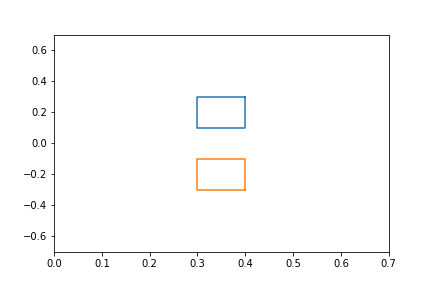
\includegraphics[width = \linewidth]{img/obstacles.png}
    \caption{Two-dimensional workspace with two obstacles}
    \label{fig:exampleWorkspace}
\end{figure}
Assume the shoulder of human arm is located at position $(0.7,0.0)$, and the robot starts at $(0.0,0.0)$. 
While the visually-impaired user in navigating freely, the system must throw an interruption command when there is a chance of collision between the human hand and an obstacle, or human arm and an obstacle. 

It would be unwise to throw an interruption only when a collision occurs, since the human may be moving very quickly and could hurt themselves. 
This means that the strategy will inevitably require some form of collision prediction. 
A simple solution to this was to apply a magnification transform on the obstacles in the workspace. 
This will throw a interruption before the arm or hand collides with the actual obstacles in the workspace. 

Using this strategy for collision detection is not optimal as it has many inherent flaws. 
For instance, in situations where there are tight spaces between obstacles, the collision detection will still throw interruptions even though no actual collision is taking place. 
Furthermore, with increased number of obstacles, this strategy significantly reduces the navigable area for the human arm. 

The experiment only tracks the motion of the human hand. 
With this information, a line segment is drawn from the predefined human shoulder location to the human hand (this method assumes that the human arm is unbending and a rigid body). 
If the segment intersects with any of the magnified obstacles in the workspace, it is taken that a collision has occurred and an interruption is thrown. 
This interruption is in the form of an auditory warning asking the human to stop their free-navigation. 
Once that is done, the human hand position and final goal position is passed to the motion planner.

\subsection{Human-Arm Conscious Motion Planner}
The goal of the motion planner is to assist the human arm in moving from a precarious position to a position closer to the goal while avoiding potential collisions with obstacles. 
First the workspace is sampled to form a navigable graph, then graph is traversed given the start and endpoint through an optimal strategy. 
Integrated into the traversal strategy is a novel cost function that evaluates if the chosen path results in collision of the human arm with obstacles. 

The assistive robot used in this experiment is a 7-DOF Sawyer robot. 
While sampling, it is important to consider if it is possible for the robot to orient itself in the sampled configuration. 
To simplify this process, first we sampled in the two-dimensional workspace and used the IK solver to determine if it is possible to orient the robot in that configuration. 
If that is not possible, a new point in the workspace and tested.  
Once the workspace is sampled, neighbours to the sampled points are determined based on the proximity (according to the euclidean distance) in both the configuration space and navigation space. 

One problem that we faced was that during sampling, there were a lot of cases when the robot could not be configured in the required orientation. 
Hence sampling of a singular point was repeated multiple times as the IK solver repeatedly threw errors. 

To navigate the graph, we use the A* algorithm for its heuristic. 
In addition to the algorithm, we added an additional cost function that evaluates if a transition to a neighbouring node is safe for the human. 
Consider two points in the graph as shown in Figure \ref{fig:humanArmConscious}. 
\begin{figure*}[htpb]
  \centering
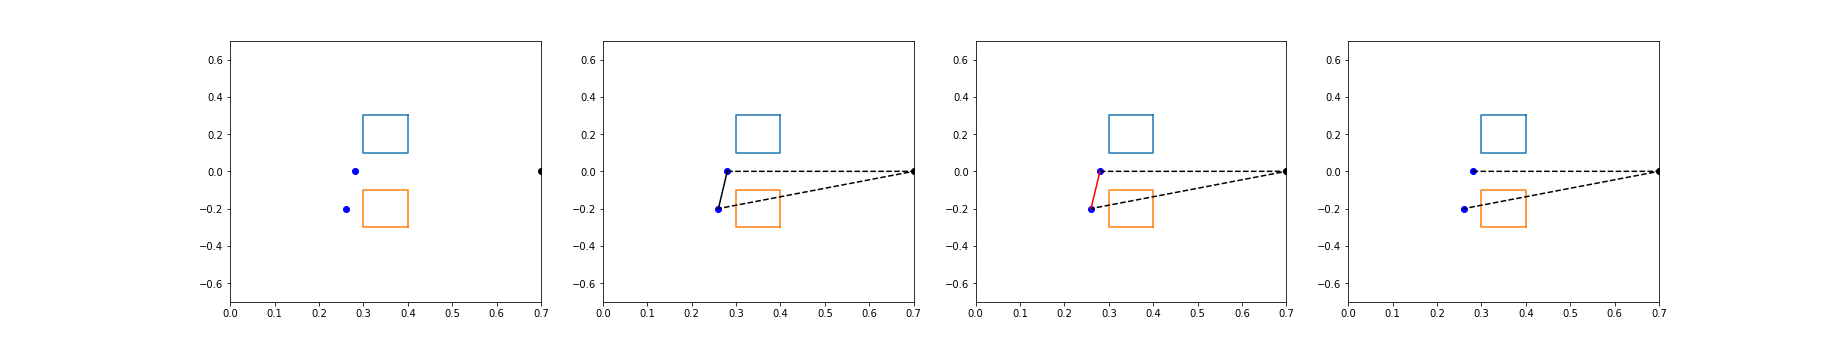
\includegraphics[width = \textwidth]{img/humanArmConscious.png}
  \caption{Human arm conscious cost function for motion planner}
  \label{fig:humanArmConscious}
\end{figure*}
We draw a polygon joining the two nodes and the human shoulder location. 
If the polygon intersects with any obstacles in the workspace, we increase the cost of transitioning between the node and its neighbour to infinity. 
This discourages the algorithm from following that transition. 

This additional cost function is rather basic and does not consider any additional properties such as arm comfort. 
It also does not take into consideration the fact that the human arm is a 2-DOF linkage that can offer greater maneuverability. 
However, it does take into consideration potential worst case scenarios and is guaranteed to provide safe trajectories. 

% Motionplanner: what is new in it? our contribution
% the platform we used and technical stuff (arm tracking method)

